%
% Complete documentation on the extended LaTeX markup used for Insight
% documentation is available in ``Documenting Insight'', which is part
% of the standard documentation for Insight.  It may be found online
% at:
%
%     http://www.itk.org/

\documentclass{InsightArticle}

\usepackage[dvips]{graphicx}
\usepackage[center]{subfigure}
\usepackage{amssymb}

%%%%%%%%%%%%%%%%%%%%%%%%%%%%%%%%%%%%%%%%%%%%%%%%%%%%%%%%%%%%%%%%%%
%
%  hyperref should be the last package to be loaded.
%
%%%%%%%%%%%%%%%%%%%%%%%%%%%%%%%%%%%%%%%%%%%%%%%%%%%%%%%%%%%%%%%%%%
\usepackage[dvips,
bookmarks,
bookmarksopen,
backref,
colorlinks,linkcolor={blue},citecolor={blue},urlcolor={blue},
]{hyperref}


%  This is a template for Papers to the Insight Journal. 
%  It is comparable to a technical report format.

% The title should be descriptive enough for people to be able to find
% the relevant document. 
\title{A VTK Algorithm for the Computation of the Hausdorff Distance}

% 
% NOTE: This is the last number of the "handle" URL that 
% The Insight Journal assigns to your paper as part of the
% submission process. Please replace the number "1338" with
% the actual handle number that you get assigned.
%
\newcommand{\IJhandlerIDnumber}{3251}

% Increment the release number whenever significant changes are made.
% The author and/or editor can define 'significant' however they like.
\release{1.0}

% At minimum, give your name and an email address.  You can include a
% snail-mail address if you like.
\author{Fr\'{e}d\'{e}ric Commandeur, J\'er\^ome Velut, Oscar Acosta}
\authoraddress{INSERM, U 642, Rennes, F-35000, France \\ Universit\'e de Rennes 1, LTSI, F-35000, France\\ frederic.commandeur@etudiant.univ-rennes1.fr \\ jerome.velut@univ-rennes1.fr\\ oscar.acosta@univ-rennes1.fr }
% Ce n'est pas pro si l'on laisse juste gmail

\begin{document}

%
% Add hyperlink to the web location and license of the paper.
% The argument of this command is the handler identifier given
% by the Insight Journal to this paper.
% 
\IJhandlefooter{\IJhandlerIDnumber}


\ifpdf
\else
   %
   % Commands for including Graphics when using latex
   % 
   \DeclareGraphicsExtensions{.eps,.jpg,.gif,.tiff,.bmp,.png}
   \DeclareGraphicsRule{.jpg}{eps}{.jpg.bb}{`convert #1 eps:-}
   \DeclareGraphicsRule{.gif}{eps}{.gif.bb}{`convert #1 eps:-}
   \DeclareGraphicsRule{.tiff}{eps}{.tiff.bb}{`convert #1 eps:-}
   \DeclareGraphicsRule{.bmp}{eps}{.bmp.bb}{`convert #1 eps:-}
   \DeclareGraphicsRule{.png}{eps}{.png.bb}{`convert #1 eps:-}
\fi


\maketitle


\ifhtml
\chapter*{Front Matter\label{front}}
\fi


% The abstract should be a paragraph or two long, and describe the
% scope of the document.
\begin{abstract}
\noindent

The Hausdorff distance is a measure of the distance between sets of points. There are many advantages to using this metric compared to other similarity measures. This document describes a VTK class for computing the Hausdorff Distance between two sets of points. The main contribution, compared to other implementations, lies in the definition of the distance not only to the closest point but to the closest point in the represented surface, which yields an accurate measure even between undersampling surfaces. This is achieved by implementing a point-to-cell distance instead of a point-to-point.  Furthermore, a plugin for ParaView was implemented, which is also available with the code. After introducing the interest of this distance, the VTK code is explained and illustrated with some examples.
%
\end{abstract}

\IJhandlenote{\IJhandlerIDnumber}

\tableofcontents

%
\section{Hausdorff distance: theoretical background}
\label{sec:hausdorff_distance}
The Hausdorff distance~\cite{HAU18.1} has been used in many applications to compute distance between sets of points. It can be used as a similarity measure for detection and tracking~\cite{Gastaldo:2002}, registration~\cite{Zhang:2005} or validation~\cite{Klein2010}. As it is based on the Euclidean norm it is dimension-independant. It is always positive and it is zero only when the shapes to be compared are the same. Our implementation builds upon the definition proposed in~\cite{ASP02} as follows.
%
\subsection{Point to surface distance definition}
%
Let $p$ a point of $\mathbb{R}^3$ and $\mathcal{S}$ a 2-dimensional surface embedded in $\mathbb{R}^3$ . The distance $\delta$ from $p$ to $\mathcal{S}$ is defined as 
%
\begin{equation}
  \delta(p,\mathcal{S}) = \inf_{q \in S} ||p - q||
\label{eq:delta}
\end{equation}
%
where $|| . ||$ corresponds to the Euclidean norm and $q$ is a point of $\mathcal{S}$. 
%
\subsection{Relative distances between two surfaces}
%
Let $\mathcal{S}_1$ and $\mathcal{S}_2$ be two 2-dimensional surfaces embedded in $\mathbb{R}^3$ and $p_1$ a point belonging to $\mathcal{S}_1$ . The equation~\eqref{eq:delta} allows to define a surface-to-surface relative distance $\Delta(\mathcal{S}_1,\mathcal{S}_2)$ as
%
\begin{equation}
  \Delta(\mathcal{S}_1,\mathcal{S}_2) = \sup_{p1 \in \mathcal{S}_1}  \delta(p1,\mathcal{S}_2)
\label{eq:Delta}
\end{equation}
%
This distance is said relative as it is not symmetrical, \textit{ie.} $\Delta(\mathcal{S}_1,\mathcal{S}_2) \ne \Delta(\mathcal{S}_2,\mathcal{S}_1)$.
%
\subsection{Hausdorff distance}
%
Finally, the Hausdorff distance $d$ between two surfaces $\mathcal{S}_1,\mathcal{S}_2$ is defined as the maximum of the two relative distances:
\begin{equation}
  d(\mathcal{S}_1,\mathcal{S}_2) = \max \left\{ \Delta(\mathcal{S}_1,\mathcal{S}_2), \Delta(\mathcal{S}_2,\mathcal{S}_1)\right\}
\end{equation}
%
\section{VTK Implementation}
%
Our Hausdorff distance implementation is designed as a \verb!vtkPointSetAlgorithm!-inherited class called \verb!vtkHausdorffDistancePointSetFilter!. It takes two \verb!vtkPointSets! as inputs: $input_A$ on input port 0 and $input_B$ on input port 1. 

Inputs are first copied on corresponding output ports. The algorithm computes then the Hausdorff distance $d(input_A,input_B)$ and the Relative distance $\Delta(input_A,input_B)$ and $\Delta(input_B,input_A)$. These distances are stored in the \verb!FieldData! of both outputs. The \verb!PointData! array of each output contain the points-to-surface distances $\delta(p_{input_A},input_B)$ and $\delta(p_{input_B},input_A)$.
%
\subsection{Target distance}
%
Although the mathematical definition of the Hausdorff distance given in section~(\ref{sec:hausdorff_distance}) is referred to $\mathbb{R}^3$  surfaces, the proposed implementation allows to perform comparisons between point sets. It is up to the user to choose which element from the compared object should be targeted: either points or cells. The choice can be made through the \verb!TargetDistanceMethod! accessors:
\begin{verbatim}
      int TargetDistanceMethod; //!< point-to-point if 0, point-to-cell if 1
      vtkSetMacro( TargetDistanceMethod, int );
\end{verbatim}
A point-to-cell distance implies the existence of cells in both inputs. This is typically the case with \verb!vtkPolyData! representing polygonal surfaces (\textit{eg.} triangulations). When such a method is used, the point-to-surface $\delta$ computation performs an geometric interpolation of the targeted cells, leading to a more precise distance calculation.  Figure~\ref{Fig:sphere-cube} illustrates the large differences between them (point-to-point and point-to-cell), considering the distance of a sphere $\mathcal{S}$ inscribed in a cube $\mathcal{C}$. A large difference appears between the two cases. In figure~\ref{Fig:sphere-cube:point-to-point_sparse-sampled}, the $\delta$ distances are computed between the sphere vertices and the cube vertices. It justifies the $\frac{\sqrt{2}}{2}$ minimum distance found in the cube face centers. In contrast, figure~\ref{Fig:sphere-cube:point-to-cell_sparse-sampled} shows that the cube face centers have a null $\delta$ thanks to the geometric interpolation.
%
\begin{figure}
\centering
\subfigure[point-to-point computation method\newline
$\Delta(\mathcal{S},\mathcal{C})=0.707$\newline
$\Delta(\mathcal{C},\mathcal{S})=0.366$\newline
$d(\mathcal{C},\mathcal{S})=0.707$\newline]{\label{Fig:sphere-cube:point-to-point_sparse-sampled} 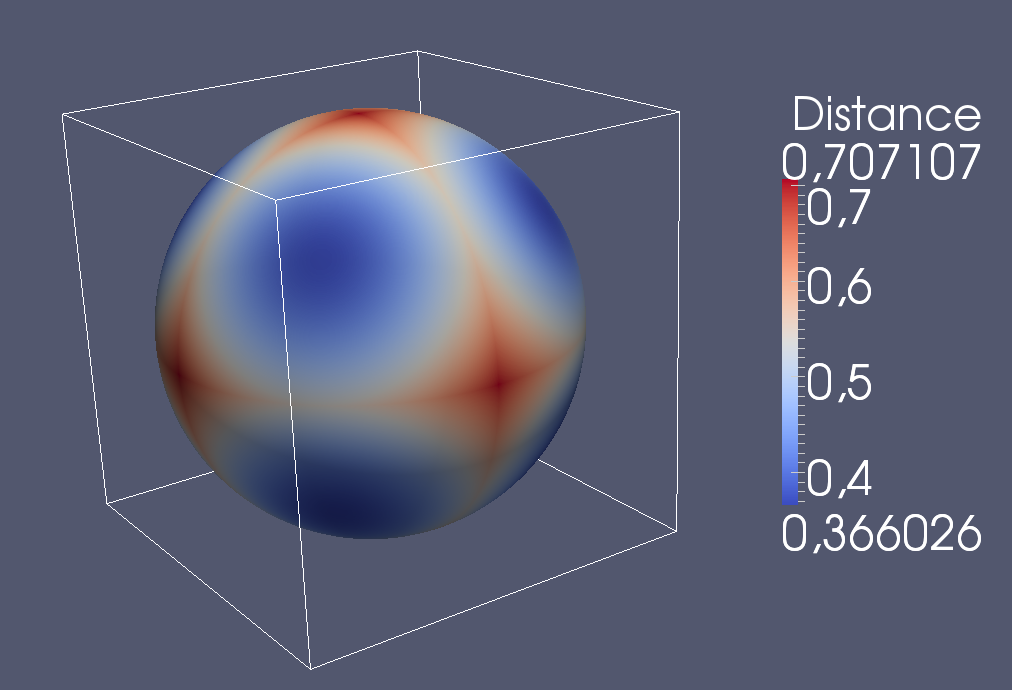
\includegraphics[width=0.4\textwidth]{./Figures/point-to-point.png}}
\hspace{0.1 \textwidth}
 \subfigure[point-to-cell computation method\newline
$\Delta(\mathcal{S},\mathcal{C})=0.211$\newline
$\Delta(\mathcal{C},\mathcal{S})=0.366$\newline
$d(\mathcal{C},\mathcal{S})=0.366$\newline]{\label{Fig:sphere-cube:point-to-cell_sparse-sampled} 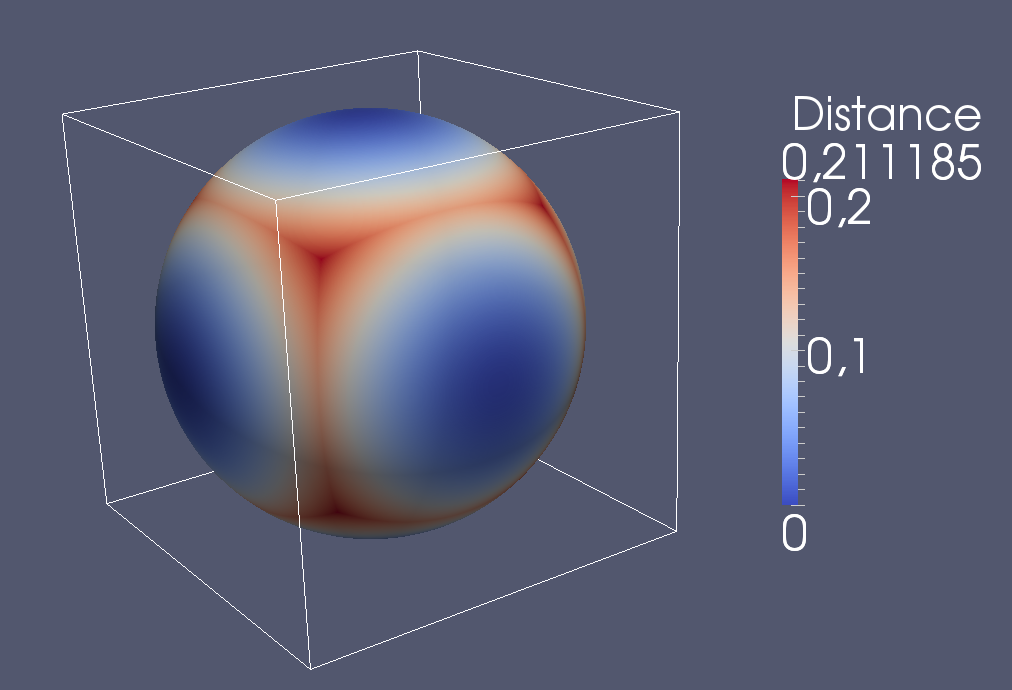
\includegraphics[width=0.4\textwidth]{./Figures/point-to-cell.png}}
\caption{Point to surface distance $\delta$ computed between a cube and its inscribed sphere}
\label{Fig:sphere-cube}
\end{figure}
%
\subsection{Computational time optimization}
%
In the Hausdorff distance computation, the bottle-neck in term of algorithmic complexity resides in the relative distances computation. Indeed, finding the minimum distance from each point $p_1$ in $\mathcal{S}_1$ to each point $p_2$ in $\mathcal{S}_2$ yield to an $\mathcal{O}(m\cdot n)$ theoretical complexity where $m$ (resp. $n$) is the number of points in $\mathcal{S}_1$ (resp. $\mathcal{S}_2$).

The proposed implementation harnesses the \verb!vtkLocator! space-partitioning classes. The minimum point-to-point distance method uses \verb!vtkKdTreePointLocator!, which decreases the complexity to $\mathcal{O}(n\log(m))$. Similarly, the point-to-surface method involved an octree space partitioning prior to minimum distance computation as implemented in \verb!vtkCellLocator!. For illustration, computing the Hausdorff distance between two point sets having each $1,000,000$ of points took $12s$ on a $2.27GHz$-cadenced processor.
%
\subsection{ParaView plugin}
%
The provided class can be build as a ParaView plugin by setting \verb!BUILD_PARAVIEW_PLUGIN! option to ON during the CMake procedure.

A \verb!vtkHausdorffDistancePointSetFilter! dynamic library will be created in the \verb!bin! directory where the \verb!ccmake! command was executed. This library is loadable from ParaView:
\begin{verbatim}
"Tools" -> "Manage Plugins" -> "Load New" -> vtkHausdorffDistancePointSetFilter.so/dll
\end{verbatim}
%
It will create a \verb!Hausdorff Distance! submenu in the \verb|Filters| menu.
%
\section{Result}
%
In this section, we show a use case of our Hausdorff distance VTK algorithm. A common task in image processing and visualisation is to extract an isosurface from a binary volume. The quality of the extracted surface will strongly depend on the resolution of the volume. In figure~\ref{fig:coarse-to-fine}, we show an extracted sphere at different coarsening levels. The Hausdorff distance from these surfaces to a ideal sphere (figure~\ref{fig:hausdorff:ref}) gives a quality measure that tends to zero when the sampling becomes finer. This is illustrated in the graph, figure~\ref{fig:hausdorff:graph}.
%
\begin{figure}
 \centering
 \subfigure[Coarsening factor 10]{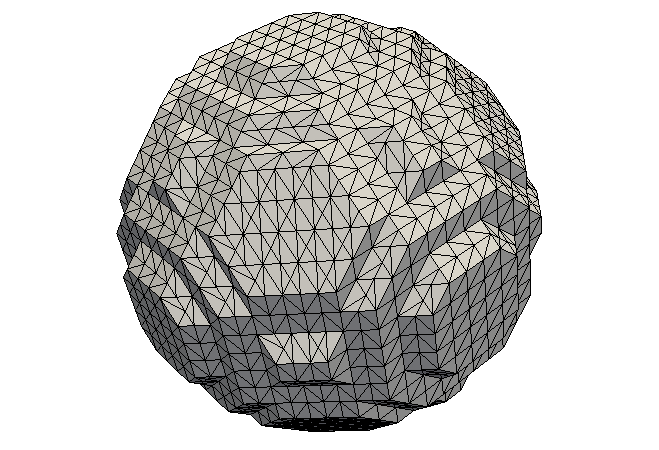
\includegraphics[width=0.49\textwidth]{./Figures/aliasing0}}
 \subfigure[Coarsening factor 8]{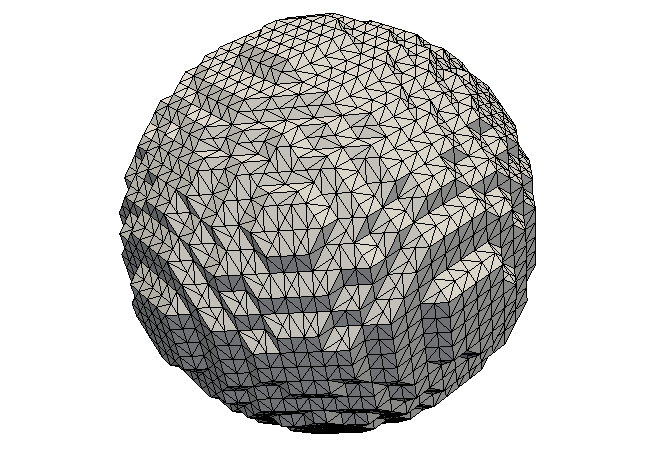
\includegraphics[width=0.49\textwidth]{./Figures/aliasing2}}
 \subfigure[Coarsening factor 6]{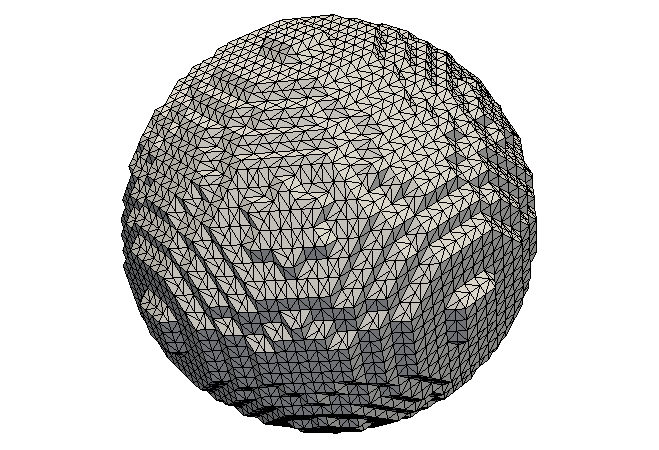
\includegraphics[width=0.49\textwidth]{./Figures/aliasing4}}
 \subfigure[Coarsening factor 4]{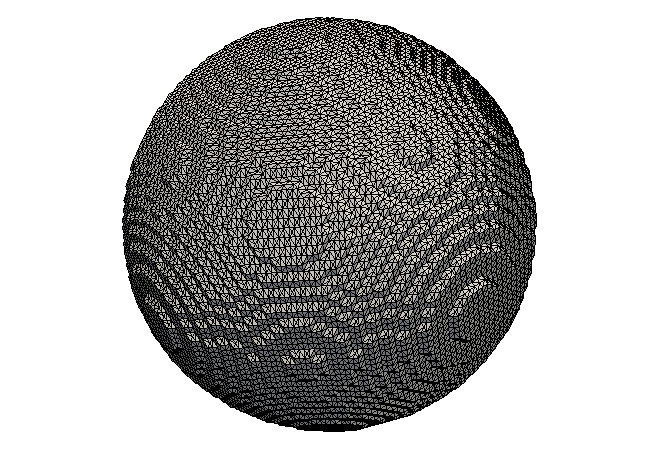
\includegraphics[width=0.49\textwidth]{./Figures/aliasing6}}
\caption{Isocontours of binary sphere with different resolutions. Initial volume (coarsening factor$ = 1$) is $512\times 512\times 512$}
\label{fig:coarse-to-fine}
\end{figure}
%
\begin{figure}
 \centering
 \subfigure[Ideal sphere]{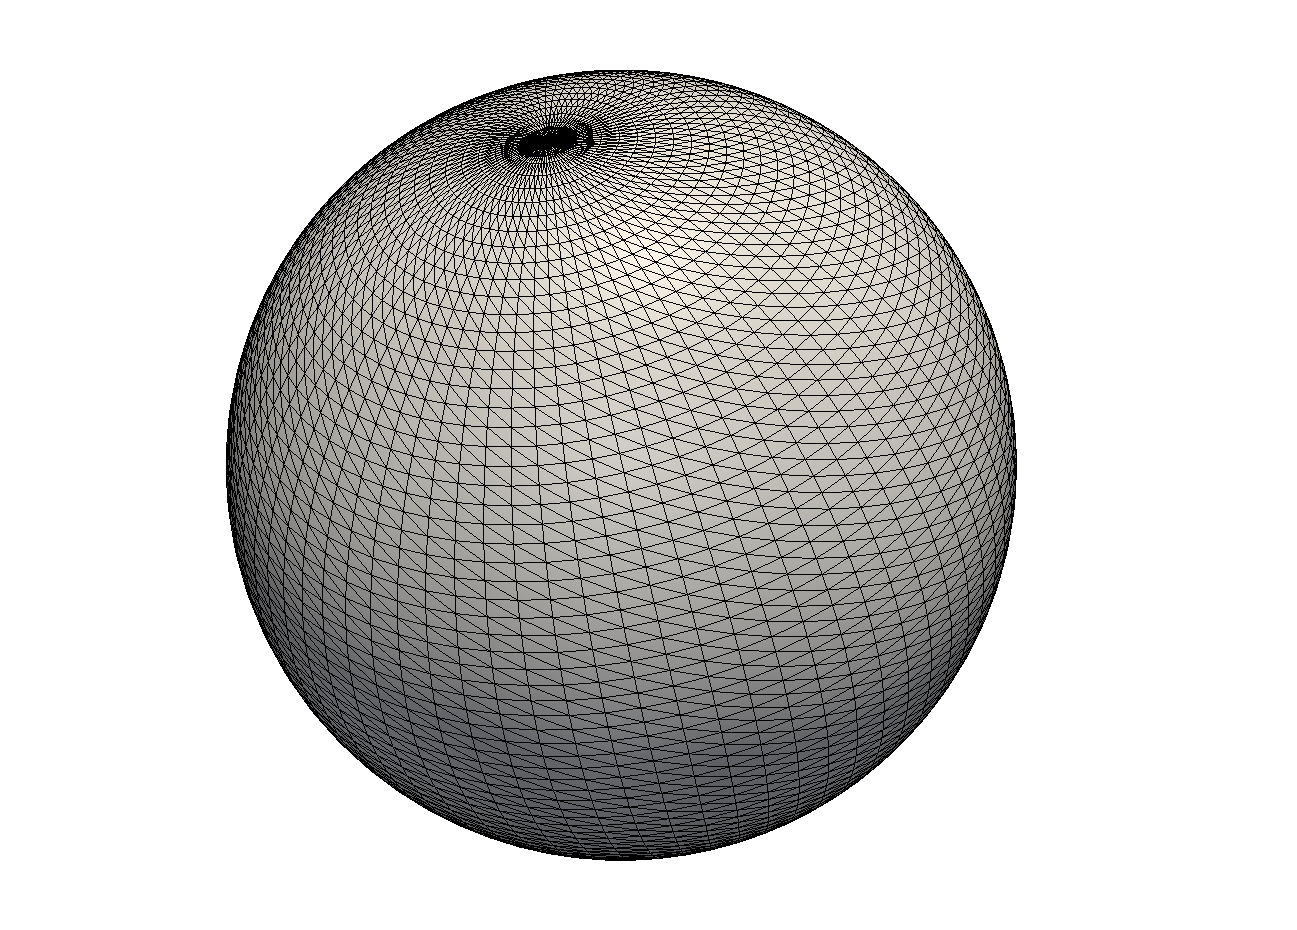
\includegraphics[width=0.49\textwidth]{./Figures/aliasing_ref}\label{fig:hausdorff:ref}}
 \subfigure[Hausdorff distance between ideal sphere and isocontours]{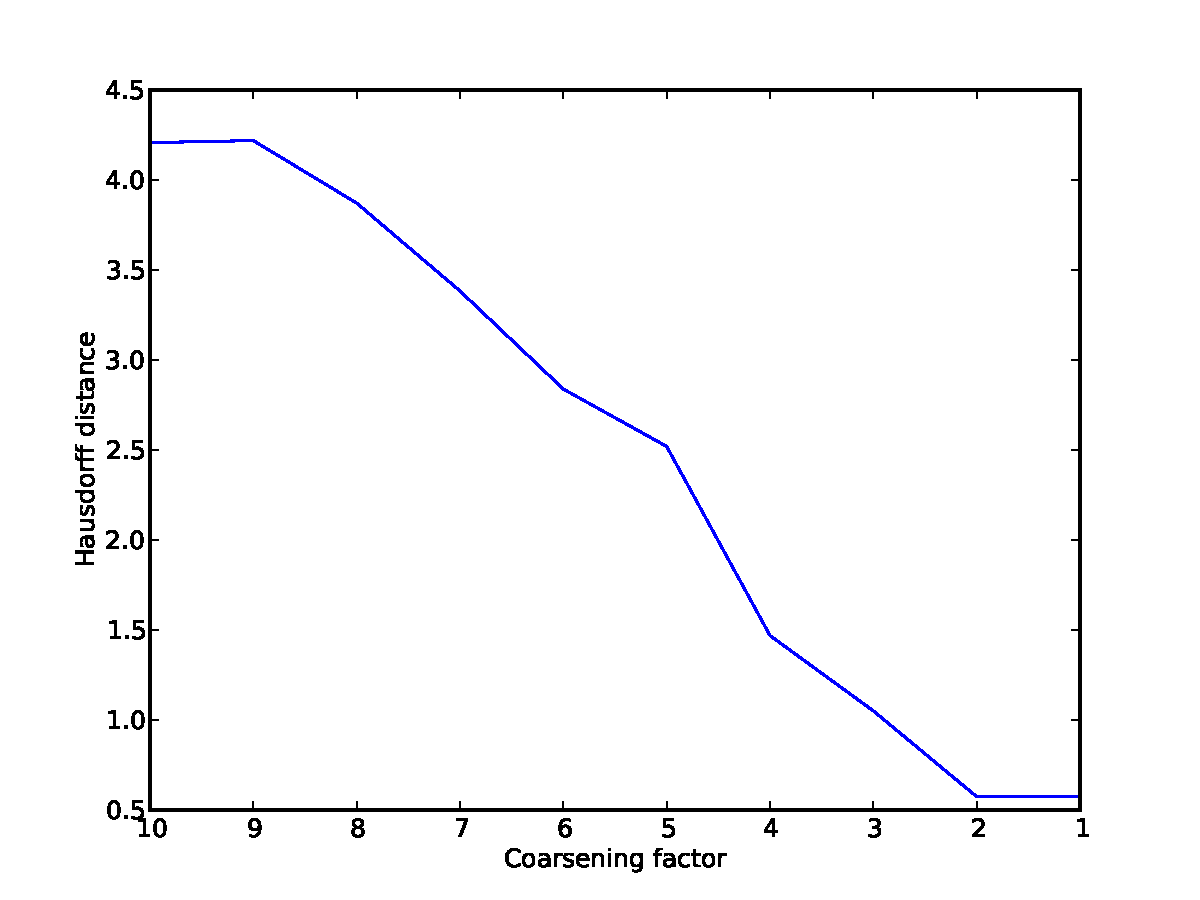
\includegraphics[width=0.49\textwidth]{./Figures/hausdorff_aliasing.pdf}\label{fig:hausdorff:graph}}
 \caption{Ideal sphere and its hausdorff distances from isocontours of figure~\ref{fig:coarse-to-fine}}
 \label{fig:hausdorff}
\end{figure}

%
\section{Software Requirements}
%
This software was built on Ubuntu 11.04 and Fedora 14 against ParaView-3.10.1, git master at the time of submission and VTK-5.6.1.
%
\section{Conclusion}
We presented a class to compute the Hausdorff distance between two point sets. This distance is appropriate to quantify the similarity of surfaces. The provided class is inherited from \verb!vtkPointSetAlgorithm! and can be executed in command line or as a ParaView plugin.
%
%
\appendix
%
%%%%%%%%%%%%%%%%%%%%%%%%%%%%%%%%%%%%%%%%%
%
%  Insert the bibliography using BibTeX
%
%%%%%%%%%%%%%%%%%%%%%%%%%%%%%%%%%%%%%%%%%
%
\bibliographystyle{plain}
\bibliography{references}
%
\end{document}

